\section{Classification and Representation}

  \subsection{Classification}
    The classification problem is just like the regression problem, except that the values we now want to predict take on only a small number of discrete values. For now, we'll discuss a binary classification problem.

  \subsection{Hypothesis Representation}
    We may use our old regression algorithm by classifying data on the basis of a threshold. But it will have very poor performance.\\ 
    \\We will introduce "Sigmoid Function", also called the "Logistic Function":
    \begin{equation}
      h_\theta(x) = g(\theta^{T}x)
    \end{equation}
    \begin{equation}
      z = \theta^{T}x
    \end{equation}
    \begin{equation}\label{eq:sigmoid}
      g(z) = \frac{1}{1+e^{-z}}
    \end{equation}
    This is how the Sigmoid Function looks like:
    \begin{figure}[h]
      \centering
      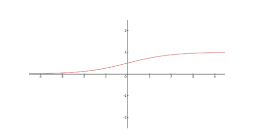
\includegraphics[scale = 0.6]{sigmoid.png}
      \caption{Sigmoid Funtion \ref{eq:sigmoid}}
    \end{figure}

  \subsection{Decesion Boundary}
    The decision boundary is the line that separates the area where y=0 and where y=1.\\
    It is similar to the decision boundary for linear regression, the only difference is the distribution of values (linear and sigmoid)

\section{Logistic Regression Model}

  \subsection{Cost Function}
    Cost funtion for logistic regression looks like:

    \begin{equation}
      J(\theta) = \frac{1}{m}\sum_{i=1}^{m}Cost(h_\theta(x^{(i)}), y^{(i)})
    \end{equation}
    \\ \\
    $ Cost(h_\theta(x),y) = -\log{(h_\theta{(x)})} $ \hfill if $y = 1$
    \\ \\
    $Cost(h_\theta(x),y) = -\log{(1-h_\theta{(x)})}$  \hfill if $y = 0$

    \begin{figure}[h]
      \centering
      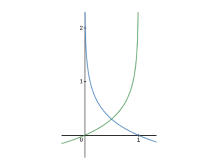
\includegraphics[scale = 0.6]{costlog.png}
      \caption{Cost Funtion}
    \end{figure}

    \subsubsection{Siplified Cost Funtion}
    This cost funtion can be compressed into a single funtion:
    \begin{equation}
      Cost(h_\theta(x),y) = -y\log{(h_\theta{(x)})} -(1-y)\log{(1-h_\theta{(x)})}
    \end{equation}
    A vectorised implementation is: \\ \\
    $h = g(X\theta)$\\
    $J(\theta) = \frac{1}{m}.(-y^T\log{h}-(1-y)^T\log{1-h})$
    \\ \\
    Vectorised implementation for Gradient Descent: \\ \\
    $\theta := \theta - \frac{\alpha}{m}X^T(g(X\theta)-y)$

\section{Multiclass Classification}
  \subsection{One-vs-all}
    This approach is when data has more than two categories.We divide our problem into n\footnote[1]{n = no of categories in dataset} binary classification problems, in each one, we predict the probability considering one of the category to be $+$ve and all other to be $-$ve. Repeating this for all other categories will finally give us all the decesion boundaries.
    \begin{figure}[h]
      \centering
      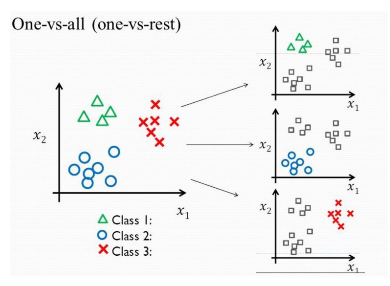
\includegraphics[scale = 0.5]{oneall.png}
      \caption{One vs all classifiaction method}
    \end{figure}   

\section{The Problem of Overfitting}
  Consider the problem of predicting y from x $\in$ R. The leftmost figure below shows the result of fitting a $y = \theta_0+\theta_1x$ to a dataset. We see that the data doesn’t really lie on straight line, and so the fit is not very good.\\ 
  \begin{figure}[h]
    \centering
    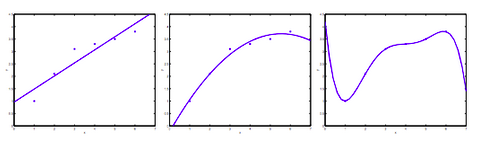
\includegraphics[scale=0.5]{overfitting.png}
  \end{figure}
  \\
  Instead, if we had added an extra feature $x^2$ , and fit $ t = \theta_0 + \theta_1x + \theta_2x^2$ , then we obtain a slightly better fit to the data (See middle figure). Naively, it might seem that the more features we add, the better. However, there is also a danger in adding too many features: The rightmost figure is the result of fitting a $5^{th}$ order polynomial $y = \sum_{j=0} ^5 \theta_j x^j$. We see that even though the fitted curve passes through the data perfectly, we would not expect this to be a very good predictor of, say, housing prices (y) for different living areas (x). Without formally defining what these terms mean, we’ll say the figure on the left shows an instance of \textbf{underfitting}—in which the data clearly shows structure not captured by the model—and the figure on the right is an example of \textbf{overfitting}.

    \subsubsection{How to address this issue?}
      \begin{enumerate}
        \item Reduce the number of features:
        \begin{itemize}
          \item Manually select which features to keep.
          \item Use a model selection algorithm.\footnote[2]{we'll cover it later}
        \end{itemize}
        \item Regularisation:
        \begin{itemize}
          \item Keep all the features, but reduce the magnitude of parameters $\theta_j$.
          \item Regularization works well when we have a lot of slightly useful features.
        \end{itemize}
      \end{enumerate}

  \subsection{Regularized Cost Function}
    To solve this problem of overfitting, we can eleminate the influence of $\theta_3x^3$ and $\theta_4x^4$. Without actually getting rid of these features or changing the form of our hypothesis, we can instead modify our cost function:
    \begin{equation}
      J_\theta = min\ of\ \left[ \frac{1}{2m} \sum_{i=1}^{m}(h_\theta(x^{(i)}) - y^{(i)})^2 + \lambda\sum_{j=1}^2\theta_j^2 \right]
    \end{equation}
    These extra terms will inflate the cost of extra parameters. \\ \\
    The $\lambda$ is called the \textbf{regularisation parameter}/ It determines how much the costs of out theta parameters are inflated.

  \subsection{Regularized Linear Regression}
    \begin{figure}[h]
      \centering
      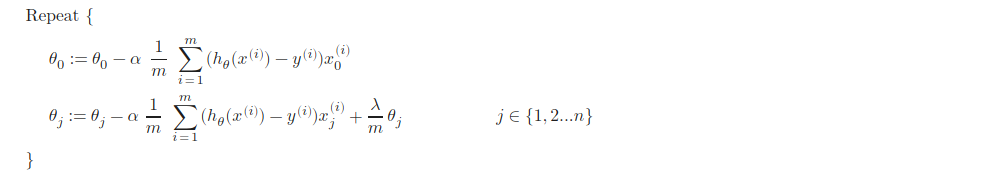
\includegraphics[scale=1]{gradregularize.png}
    \end{figure}


    The term $\frac{\lambda}{m}\theta_{j}$ performs our regularization. With some manipulation, our update rule can also be represented as \\

    $ \theta_j := \theta_j(1 - \alpha\frac{\lambda}{m}) - \alpha\frac{1}{m}\sum_{i=1}^m(h_\theta(x^{(i)}) - y^{(i)})x_j^{(i)} $\\

    The first term in the above equation, $\alpha\frac{\lambda}{m}$ will always be less than 1. Intuitively you can see it as reducing the value of $j\theta_j$ by some amount on every update.

    \subsubsection{Normal Eequation}
      This will be the non-iterative approach for regularisation.\\\\
      To add in regularization, we'll just add another term:
      \begin{equation}
        \theta = X^T X + \lambda . L^{-1} X^T y
      \end{equation}
      where, L is $(n+1)\times(n+1)$ matrix with 0 at the top lest, 1`s down the diagonal and all other element '0'.
    % \\ \\
    % \lstinputlisting[language=Octave, caption=Octave Implementation for Logistic Regression Algorithms]{logisticRegression.m}
